\documentclass[ngerman,a4paper]{article}

\usepackage{babel}
\usepackage{amsthm}
\usepackage{amsmath}
\usepackage{amssymb}
\usepackage{tikz,tkz-euclide}
\usepackage{titlesec}
\usepackage[titles]{tocloft}
\usepackage{csquotes}

\usetkzobj{all}
\usetikzlibrary{shapes.misc}

\MakeOuterQuote{"}

\newcommand*\circled[1]{%
  \tikz[baseline=(C.base)]\node[draw,circle,inner sep=0.75pt](C) {#1};\!
}

\renewcommand{\thesubsection}{\arabic{subsection}}
\titleformat{\section}{\normalfont\Large\bfseries}{Kapitel \arabic{section}: }{0em}{}
\titleformat{\subsection}{\normalfont\large\bfseries}{§\arabic{subsection} }{0em}{}
\titleformat{\subsubsection}{\normalfont\bfseries}{\arabic{subsection}.\arabic{subsubsection} }{0em}{}
\renewcommand{\cftsubsecpresnum}{§}
\newlength\mylength
\settowidth\mylength{\cftsubsecpresnum}
\settowidth\mylength{\cftsubsecaftersnum}
\addtolength\cftsubsecnumwidth{\mylength}
\renewcommand{\cftsecpresnum}{Kapitel }
\renewcommand{\cftsecaftersnum}{: }
\settowidth\mylength{\cftsecpresnum}
\addtolength\cftsecnumwidth{\mylength}

\renewcommand{\qed}{\begin{flushright}
\underline{\(q.e.d.\)}
\end{flushright}}

\title{Lineare Algebra II: Skript}
\author{Nico Mexis}
\date{\today}

\begin{document}
\maketitle
\newpage

\tableofcontents
\newpage

\setcounter{section}{4}
\section{Endomorphismen}
\setcounter{subsection}{17}
\subsection{Eigenwerte (Buch: §4.1-4.2)}
Sei \(K\) ein Körper.\\
Sei \(V\) ein endlich dimensionaler \(K\)-Vektorraum.\\
Sei \(\phi: V \rightarrow V\) ein Endomorphismus.
\subsubsection{Definition}
\begin{description}
\item[\circled{a}] Ein Element \(\lambda \in K\) heißt ein \underline{Eigenwert} von \(\phi\), wenn es einen Vektor \(v \in V\ \backslash \{0\}\) gibt mit \(\phi(v)=\lambda*v\).
\item[\circled{b}] Ist \(\lambda \in K\) ein Eigenwert von \(\phi\), so heißt jeder Vektor \(v \in V \backslash \{0\}\) mit \(\phi(v) = \lambda*v\) ein Eigenvektor von \(\phi\) zum Eigenwert \(\lambda\).
\item[\circled{c}] Ist \(A \in Mat_n(K)\), so heißt ein \(\lambda \in K\) ein \underline{Eigenwert} von A, wenn es ein \(v \in K^n\backslash\{0\}\) gibt mit \(A*v=\lambda*v\).
\end{description}
\subsubsection{Beispiel}
\begin{description}
\item[\circled{a}] Das Element \(0 \in K\) ist ein Eigenwert von \(\phi\), wenn \(\phi\) nicht injektiv ist.
\item[\circled{b}] Das Element \(1 \in K\) ist ein Eigenwert von \(\phi\), wenn \(\phi\) einen \underline{Fixpunkt} \(v \neq 0\) hat (d.h. \(\phi(v)=v\)).
\end{description}
\subsubsection{Beispiel}
Sei \(K = \mathbb{R}, V= \mathbb{R}^2\).\\
Sei \(\phi:\mathbb{R}^2\rightarrow\mathbb{R}^2\) die Drehung um \(0=(0,0)\) um den Winkel \(\alpha \in [0,2\pi[\).\\
\begin{description}
\item[\circled{a}] Ist \(\alpha = 0\), so ist \(\phi = id_{\mathbb{R}^2}\) und \(\lambda = 1\) ist der einzige Eigenwert von \(\phi\).
\item[\circled{b}] Ist \(\alpha = \pi\), so ist \(\phi = -id_{\mathbb{R}^2}\) und \(\lambda = -1\) ist der einzige Eigenwert von \(\phi\).
\item[\circled{c}] Ist \(\alpha \notin \{0,\pi\}\), so besitzt \(\phi\) keine Eigenwerte.
\end{description}
\subsubsection{Beispiel}
Sei \(K = \mathbb{R}, V= \mathbb{R}^2\) und \(\sigma :\mathbb{R}^2 \rightarrow\mathbb{R}^2\) die Spiegelung an der Geraden \(G\) durch \(0\), die mit der x-Achse einen Winkel \(\frac{\alpha}{2}\) einschließt.\newpage
\underline{Skizze:}\\
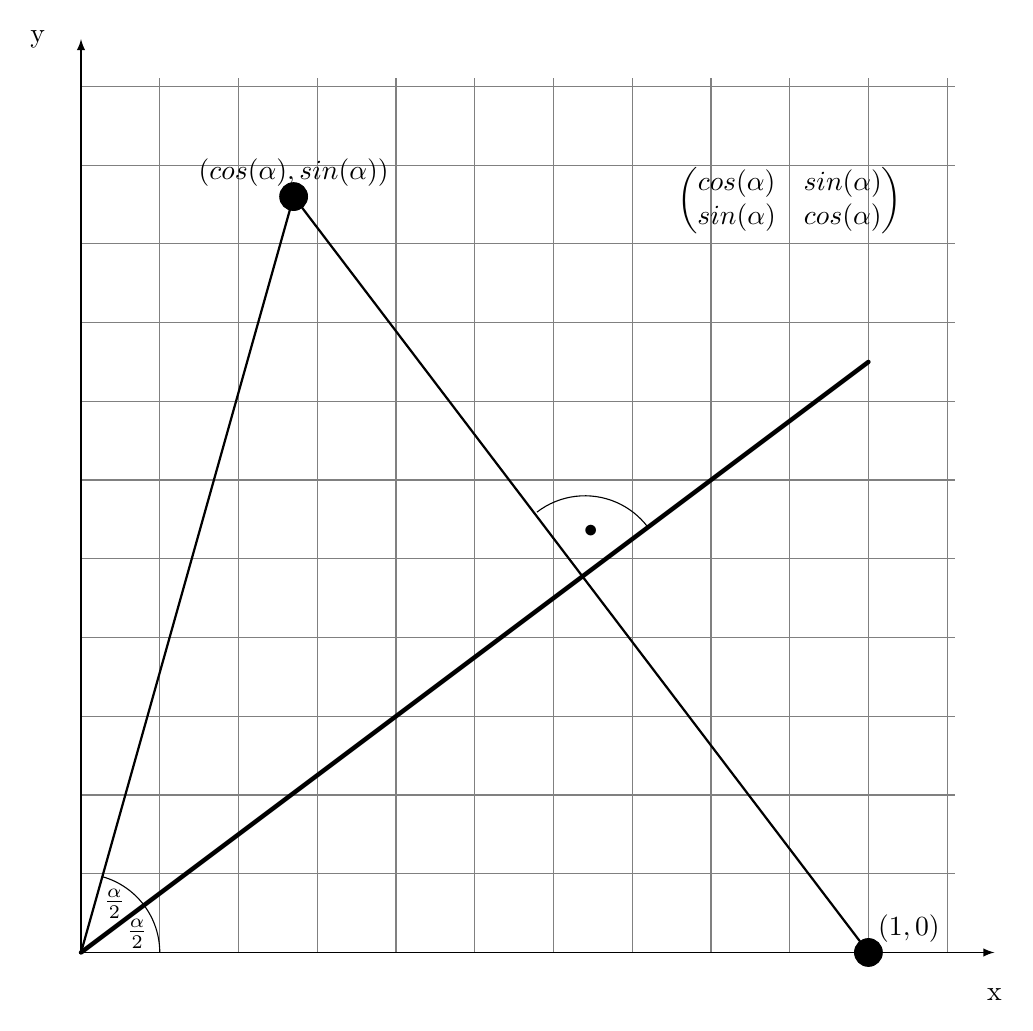
\begin{tikzpicture}
  \tkzInit[ymin=0,ymax=1.11,xstep=0.1,ystep=0.1,xmin=0,xmax=1.11]
  \tkzGrid
  \tkzLabelX
  \tkzLabelY
  \tkzDrawX[below=12 pt,label={x}]
  \tkzDrawY[left=12 pt,label={y}]
  \tkzDefPoint(1,0){V}
  \tkzDefPoint(0,0){S}
  \tkzDefPoint(0.9,0.9){P}
  \tkzDefPoint(1, 0.75){T}
  \tkzDefPoint(0.27, 0.96){U}
  \tkzDefPoint(0.64, 0.48){E}
  \tkzSetUpPoint[size = 10]
  \tkzDrawPoints[fill=black](V,U)
  \tkzLabelPoint[above](U){\((cos(\alpha),sin(\alpha))\)}
  \tkzLabelPoint[above right](V){\((1,0)\)}
  \tkzDrawSegment[ultra thick,black](S,T)
  \tkzDrawSegment[thick,black](U,V)
  \tkzDrawSegment[thick,black](S,U)
  \tkzMarkAngle(T,E,U)
  \tkzLabelAngle[pos=0.55](T,E,U){\(\bullet\)}
  \tkzMarkAngle(T,S,U)
  \tkzLabelAngle[pos=0.75](T,S,U){\(\frac{\alpha}{2}\)}
  \tkzMarkAngle(V,S,T)
  \tkzLabelAngle[pos=0.75](V,S,T){\(\frac{\alpha}{2}\)}
  \tkzLabelPoint[above](P){\(\begin{pmatrix}
cos(\alpha) & sin(\alpha) \\
sin(\alpha) & cos(\alpha)
\end{pmatrix}\)}
\end{tikzpicture}\\\\
Ein Eigenwert ist \(\lambda=1\) und die Menge der Eigenvektoren zum Eigenwert \(\lambda=1\) ist \(G\backslash\{0\}\).\\
Ein weiterer Eigenwert ist \(\lambda=-1\) und die Menge der Eigenvektoren zum Eigenwert \(\lambda=-1\) ist \(H\backslash\{0\}\), wobei \(H\) die zu \(G\) senkrechte Gerade durch 0 ist.
\subsubsection{Definition}
Sei \(\lambda \in K\) ein Eigenwert von \(\phi\). Dann heißt \(Eig(\phi,\lambda)=\{v \in V | \phi (v)=\lambda *v\}\) der \underline{Eigenraum} zum Eigenwert \(\phi\).
\subsubsection{Satz}
Sei \(\phi:V \rightarrow V\) ein Endomorphismus.
\begin{description}
\item[\circled{a}] Ist \(\lambda \in K\) ein Eigenwert von \(\phi\), so ist \(Eig(\phi,\lambda)\) ein Untervektorraum von V.
\item[\circled{b}] Sind \(\lambda,\mu \in K\) zwei verschiedene Eigenwerte von \(\phi\), so gilt: \(Eig(\phi,\mu)=\{0\}\).
\end{description}
\newpage
\underline{Beweis:}
\begin{description}
\item["\circled{a}"] Wegen \(\phi(0)=\lambda*0=0\) gilt \(\phi(v-w)=\phi(v)-\phi(w)=\lambda*v-\lambda*w=\lambda*(v-w)\), also \(v-w \in Eig(\phi,\lambda)\). Nach dem Untervektorraumkriterium folgt die Behauptung.
\item["\circled{b}"] Sei \(v \in Eig(\phi,\lambda)\cap Eig(\phi,\mu)\). Dann gilt \(\lambda*v=\phi(v)=\mu*v\), also \(\underbrace{(\lambda-\mu)}_{\neq 0}*v=0\). Dies liefert \(v=0\).
\end{description}
\qed

\end{document}






























